\documentclass[final,t]{beamer}
\mode<presentation>
{
%  \usetheme{Warsaw}
%  \usetheme{Aachen}
%  \usetheme{Oldi6}
%  \usetheme{I6td}
  \usetheme{I6dv}
%  \usetheme{I6pd}
%  \usetheme{I6pd2}
}
% additional settings
\setbeamerfont{itemize}{size=\normalsize}
\setbeamerfont{itemize/enumerate body}{size=\normalsize}
\setbeamerfont{itemize/enumerate subbody}{size=\normalsize}

\usepackage{wrapfig}
% additional packages
\usepackage{times}
\usepackage{amsmath,amsthm, amssymb, latexsym}
\usepackage{exscale}
%\boldmath
\usepackage{booktabs, array}
%\usepackage{rotating} %sideways environment
\usepackage[english]{babel}
\usepackage[latin1]{inputenc}
\usepackage[orientation=landscape,size=a1,scale=1.15]{beamerposter}
\listfiles
\graphicspath{{figures/}}
% Display a grid to help align images
%\beamertemplategridbackground[1cm]

\title{\huge Physical Travelling Salesman Problem}
\author{Sander Siim, Karl Tarbe}
\institute[University of Tartu]{Institute of Computer Science, University of Tartu, Tartu, Estonia}
\date[Dec. 18 , 2014]{Dec. 18 , 2014}

% abbreviations
\usepackage{xspace}
\makeatletter
\DeclareRobustCommand\onedot{\futurelet\@let@token\@onedot}
\def\@onedot{\ifx\@let@token.\else.\null\fi\xspace}
\def\eg{{e.g}\onedot} \def\Eg{{E.g}\onedot}
\def\ie{{i.e}\onedot} \def\Ie{{I.e}\onedot}
\def\cf{{c.f}\onedot} \def\Cf{{C.f}\onedot}
\def\etc{{etc}\onedot}
\def\vs{{vs}\onedot}
\def\wrt{w.r.t\onedot}
\def\dof{d.o.f\onedot}
\def\etal{{et al}\onedot}
\makeatother

%%%%%%%%%%%%%%%%%%%%%%%%%%%%%%%%%%%%%%%%%%%%%%%%%%%%%%%%%%%%%%%%%%%%%%%%%%%%%%%%%%%%%%%%%%%%%%%%%%%%%%%%%%%%
%%%%%%%%%%%%%%%%%%%%%%%%%%%%%%%%%%%%%%%%%%%%%%%%%%%%%%%%%%%%%%%%%%%%%%%%%%%%%%%%%%%%%%%%%%%%%%%%%%%%%%%%%%%%
\begin{document}
\begin{frame}{} 
  \begin{columns}[t]
    \begin{column}{.305\linewidth}

      %%%%%%%%%%%%%%%%%%%%%%%%%%%%%%%%%%%%%%%%%%%%%%%%%%%%%%%%%%%%%%%%%%%%%%%%%%%%%%%%%%%%%%%%%%%%%%%%%%%%%%%%%%%%

      \begin{block}{Introduction}
        The \alert{physical travelling salesman problem} (PSTP) is an abstraction into the physical world of the well-known travelling salesman optimization problem.
        \vskip1ex

        \begin{itemize}
        \item In regular TSP, the objective is to find a \alert{Hamiltonian path} in a weighted graph with minimum total cost.
        \item In PSTP, the goal is to \alert{minimize the time} that it takes to follow the trajectory of the Hamiltonian path, taking into account \alert{physical laws of motion}.
        \item Solutions for TSP are in general \alert{not optimal} for PSTP, since force needs to be applied to change direction of motion and sharp turns are costly.
        \end{itemize}
      \end{block}

      %%%%%%%%%%%%%%%%%%%%%%%%%%%%%%%%%%%%%%%%%%%%%%%%%%%%%%%%%%%%%%%%%%%%%%%%%%%%%%%%%%%%%%%%%%%%%%%%%%%%%%%%%%%%
      
      \begin{block}{GECCO 2005 PTSP Competition}
        We followed the problem statement from GECCO'05 conference PTSP competition. 
        \begin{columns}[T]
          \begin{column}{.53\linewidth} 
            \begin{figure}
              \centering
              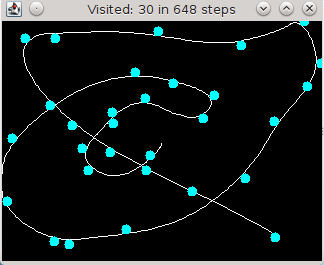
\includegraphics[width=\linewidth]{byrod_solution1.png}          
              \caption{GECCO'05 competition winner Martin Byr\"{o}d's solution}
            \end{figure}
          \end{column}

          \begin{column}{.39\linewidth} 
            \begin{figure}
              \centering
              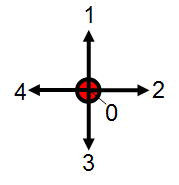
\includegraphics[width=\linewidth]{directions.png}          
              \caption{One of 5 force vectors are applied at every time step}
            \end{figure}
          \end{column}
          
        \end{columns}
        \vskip1ex

        Salesman has a mass of 1 kg. At every time step ($dt = \sqrt{0,1}$), force of 1N can be applied to
        salesman in either X or Y axis. Newton's equations for velocity and displacement are used for the simulation.
        Cities are placed in 320x240 grid and each has a radius of 5m.

        \begin{itemize}
            \item All best solutions used genetic algorithms.
            \item No crossover was used, only mutations.
            \item Most tried to first find a suitable route for visiting the cities and then optimize the corresponding trajectory. 
            %\item Some optimize the route incrementally.
        \end{itemize}

        \vskip-1.2ex
        % \begin{columns}[T]
        %   \begin{column}{.49\linewidth}
        %     \begin{itemize}
        %     \item \alert{similar to speech recognition}: temporal sequences of images
        %     \item important features
        %       \begin{itemize}
        %       \item hand-shapes, facial expressions, lip-patterns
        %       \item orientation and movement of the hands, arms or body
        %       \end{itemize}
        %     \item HMMs are used to compensate time and amplitude variations of the signers\par
        %       \vskip2ex              
        %       %\centerline{\includegraphics[width=.5\linewidth]{dreuw/hmm}}
        %     \end{itemize}
        %   \end{column}
        %   \begin{column}{.49\linewidth}
        %     \begin{itemize}
        %     \item \alert{goal:} find the model which best expresses the observation sequence
        %     \end{itemize}
        %     \vskip2ex
        %     %\includegraphics[width=\linewidth]{dreuw/xfigures/BayesArchitectureSignLanguage_Dreuw_01Jun06}
        %   \end{column}
        % \end{columns}
      \end{block}

    
      %%%%%%%%%%%%%%%%%%%%%%%%%%%%%%%%%%%%%%%%%%%%%%%%%%%%%%%%%%%%%%%%%%%%%%%%%%%%%%%%%%%%%%%%%%%%%%%%%%%%%%%%%%%%

    \end{column}
    \begin{column}{.305\linewidth}
      \begin{block}{Our Approach}
        Similarly to GECCO'05 competition, we divide the problem into \alert{two phases}. In the first phase, we find an optimal \alert{route for visiting} all the cities. In the second phase, we optimize the \alert{corresponding trajectory} \ie the sequence of applied force vectors. We also use an evolutionary approach in both phases.
        \vskip1ex
        \noindent{\textbf{Finding optimal route}}
        
        TSP solutions do not give good results. Need a different heuristic. Explaing heuristic and genetic algorithm.

        Need nice picture with circle's to illustrate trajectory estimation.

        \vskip1ex
        \noindent{\textbf{Generating optimal trajectory}}
        
        We have good route. Need to generate trajectory with force vectors. Explain PID-controller and genetic algorithm.

        Several approaches were tried. The first was to use a \alert{proportional-integral-derivative} (PID) controller.
        The reasoning was, that this.

      \end{block}

      % \begin{block}{Feature Selection and Model Combination}
      %   \begin{columns}[T]
      %     \begin{column}{.35\linewidth}
      %       \noindent{\hskip1cm\textbf{Feature Selection}}\par
      %       \begin{itemize}
      %       \item \alert{concatenation} of appearance-based and manual features
      %       \item \alert{sliding window} for context modeling
      %       \item \alert{dimensionality reduction} by PCA and/or LDA
      %       \end{itemize}
      %     \end{column}
      %     \begin{column}{.65\linewidth}
      %       \raggedleft
      %       %\includegraphics[width=.95\linewidth]{images/xfigures/CompositeFeature_Dreuw_28Sep06}%
      %     \end{column}
      %   \end{columns}

      %   \vskip5ex
      %   \begin{columns}[T]
      %     \begin{column}{.35\linewidth}
      %       \noindent{\hskip1cm\textbf{Model Combination}}\par
      %       \begin{itemize}
      %       \item \alert{log-linear combination} of independently
      %         trained models
      %       \item profit from independent alignments (\eg performing well for long and short words)
      %       \item profit from different feature extraction approaches
      %       \end{itemize}
      %     \end{column}
      %     \begin{column}{.65\linewidth}
      %       \raggedleft
      %       %\includegraphics[width=\linewidth]{images/xfigures/CompositeModels_Dreuw_17Apr07}
      %     \end{column}
      %   \end{columns}


        %%%%%%%%%%%%%%%%%%%%%%%%%%%%%%%%%%%%%%%%%%%%%%%%%%%%%%%
      % \end{block}

    \end{column}

    %%%%%%%%%%%%%%%%%%%%%%%%%%%%%%%
    
    \begin{column}{.305\linewidth}

      \begin{block}{Results of Our Algorithm}
        %%%%%%%%%%%%%%%%%%%%%%%%%%%%%%%%%%%%%%%%%%%%%%%%%%%%%%%
        
        How well did we do compared to others?
      \end{block}
      
  
        
                
      \begin{block}{Conclusion}
        \begin{itemize}
        \item Blah blah
        \item BLah blah
        \end{itemize}
        \vspace{-1ex}
      \end{block}
%%%%%%%%%%%%%%%%%%%%%%%%%%%%%%%%%%%%%%%%%%%%%%%%%%%%%%%

    \end{column}
  \end{columns}
\end{frame}

\end{document}


%%%%%%%%%%%%%%%%%%%%%%%%%%%%%%%%%%%%%%%%%%%%%%%%%%%%%%%%%%%%%%%%%%%%%%%%%%%%%%%%%%%%%%%%%%%%%%%%%%%%
%%% Local Variables: 
%%% mode: latex
%%% TeX-PDF-mode: t
%%% End: 
